\chapter{Turbulencia, campos eléctricos e islas magnéticas}
\section{Introducción}
De cara a la viabilidad de un reactor es necesario que las reacciones de fusión que se
produzcan se sostengan sin necesidad de aportar energía al sistema, esto se conoce como ignición. 
Para conseguir la ignición es necesario que se cumpla la ley de Lawson~\eqref{eq:lawson}. Dicha
ley establece un mínimo en el producto densidad $(n)$, tiempo de confinamiento
de energía $(\tau_e)$ y temperatura $(T)$.
Para alcanzar ese valor mínimo del triple producto existen dos caminos: el primero de ellos consiste
en incrementar el tamaño de la máquina, de forma que se incremente tanto la densidad como
el tiempo de confinamiento. El inconveniente de este es fundamentalmente económico, ya
que el precio de un reactor de fusión es directamente proporcional a su tamaño. El segundo
modo de alcanzar el triple producto consiste en incrementar el tiempo en el que permanecen
confinadas las partículas y la energía. Los plasmas son un medio altamente turbulento, lo que
implica un alto transporte radial de partículas y energía y como consecuencia un bajo tiempo
de confinamiento. Una reducción de la turbulencia aumentaría el tiempo de confinamiento y
por tanto el triple producto para alcanzar la ignición. Esta forma de conseguir ignición en un
futuro reactor es más económica.\par
La primera aproximación para entender la turbulencia en el plasma, viene de la descripción 
de la turbulencia en fluidos neutros. La descripción matemática de los fluidos tanto en
régimen laminar como en régimen turbulento viene dada por la ecuación de Navier-Stokes.
Para clasificar el régimen del fluido, se puede utilizar el número de Reynolds (Re); permite
clasificar el régimen turbulento de un fluido por encima de un valor crítico. Por debajo
de dicho valor el fluido se encuentra en régimen laminar. El número de Reynolds se define:
\begin{equation}\label{eq:reynolds}
    Re=\frac{v_s\cdot D}{\nu}
\end{equation}
done $v_s$ es la velocidad característica del fluido, D es la longitud característica del sistema y
$\nu$ es la viscosidad cinemática. En fluidos neutros no solo una elevada velocidad puede desencadenar
un régimen turbulento, sino que determinadas inestabilidades pueden ser también
causantes de la turbulencia (las inestabilidades que pueden provocan la turbulencia en plasmas de
fusión se comentan en~\ref{subsec:turbgen}).
Los plasmas de fusión se contemplan como una mezcla de dos fluidos (iones y electrones). No
se pueden considerar como un fluido neutro ya que tienen carga eléctrica, no son isótropos
dado que en la dirección del campo magnético tienen un comportamiento distinto al del resto
de direcciones y no son homogéneos dado que poseen fuertes gradientes de densidad, temperatura,
etc. Todo ello hace que en los plasmas de fusión la variedad de inestabilidades sea
mayor que en los fluidos neutros, lo que los convierte en un medio por sí mismo turbulento.
\subsection{Espectro de la turbulencia}
Una forma de caracterizar la turbulencia es mediante su espectro en número de onda.
Cuando se estudia un campo turbulento, se pueden encontrar remolinos (\textit{eddies}) de distintos
tamaños, es lo que se conoce como escalas de la turbulencia. Cada una de esas estructuras
posee un frecuencia y una energía.
Uno de los modelos que mejor describen la turbulencia fue propuesto por Kolmogorov en
1941~\cite{20000584634}. Dicho modelo arroja fundamentalmente tres resultados:
\begin{itemize}
    \item El modelo de cascada de la energía.
    \item La ley de disipación de energía.
    \item La ley $-5/3$ del espectro de energía.
\end{itemize}
El modelo de cascada de energía fue enunciado por F.L. Richardson en 1922~\cite{richardson_lynch_2007} y formalizado
por Kolmogorov en 1941\cite{20000584634}. Parte de determinadas hipótesis, una de ellas es la hipótesis de
transferencia de energía, la cual supone que la energía cinética se transfiere desde las grandes
escalas hacia las más pequeñas.
En la figura~\ref{fig:espectro} se puede ver el espectro en número de onda de la turbulencia. El modelo
K-41 establece dos partes en dicho espectro. En primer lugar existe una escala $l_0$ que es a la
cual se inyecta energía en el sistema.
A medida que aumenta el número de onda $k$, entramos en el intervalo de inercia en el que
las estructuras turbulentas pueden tener distintos tamaños. Esto sucede porque las estructuras
iniciales $l_0$ se van rompiendo en estructuras cada vez más pequeñas, produciéndose una
transferencia de energía cinética. A este rango de escalas de la turbulencia se las denomina
$l_T$. El último rango del espectro de la turbulencia, es lo que se conoce como el rango de
disipación. En este rango, el tamaño de las estructuras es muy pequeño $l_D$ y por lo tanto la
viscosidad del fluido comienza a tener un efecto notable en lo que respecta a disipación de
energía. Para cuantificar la conversión de energía mecánica en térmica, se utiliza la tasa de
transferencia de energía $\varepsilon$, cuyas unidades son energía por unidad de masa por segundo.
Otra de las hipótesis que se siguen en la teoría K-41 es la ley de universalidad de Kolmogorov,
la cual supone que la energía contenida en un número de onda $k_i$, es proporcional a su tasa $\varepsilon$. 
La energía para un número de onda $k$ viene dada por:
\begin{equation}\label{eq:k41}
    E(k)=C\cdot\varepsilon^{\alpha}\cdot k^\beta
\end{equation}
Donde C es una constante adimensional, $\varepsilon$ es el coeficiente de la tasa de transferencia de
energía, en función del número de onda $k$ en el que se encuentre el intervalo a estudiar. En
el intervalo de inercia, según la ley de Kolmogorov el espectro se comporta según 
$E(k)\approx C\cdot\varepsilon^{2/3}\cdot k^{-5/3}$ y en el rango de disipación 
se determinó experimentalmente que $E(k)=Ck^{-N}$, donde $N>5/3$.
\begin{figure}
    \centering
    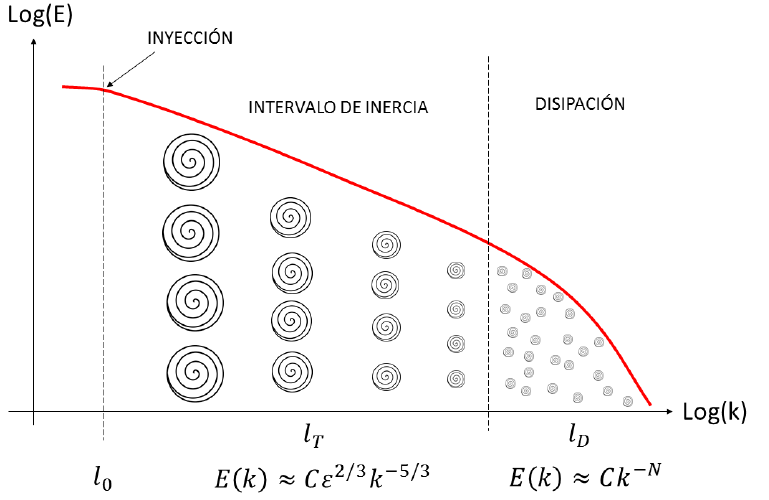
\includegraphics[scale=0.5]{img/espectro.png}
    \caption{Espectro de la turbulencia según la teoría K-41.}
    \label{fig:espectro}
\end{figure}
\subsection{Generación de la turbulencia}\label{subsec:turbgen}
La turbulencia suele estar producida por fuentes de energía libre tales como los gradientes,
las corrientes, etc. y puede estar presente en distintas magnitudes como campos eléctricos,
campos magnéticos, densidad, temperatura, etc. 
Un modelo ampliamente aceptado de las inestabilidades que inician la turbulencia en el
plasma es el modelo de inestabilidad producido por ola de deriva. Esta inestabilidad se inicia 
cuando se produce
una fluctuación de densidad tridimensional. Los electrones
reaccionarán primero al gradiente de densidad (electrones más rápidos que los iones debido
a la diferencia de masa) abandonando esa región antes que los iones y haciendo que esta
quede cargada positivamente. La dirección en la cual existe la perturbación quedará cargada
positiva y negativamente de forma alternada, lo que generará un potencial electrostático y
por lo tanto un campo eléctrico. Este campo
eléctrico conlleva un deriva $\vec{E}\times\vec{B}$, 
que amplificará la perturbación. Por otra parte la deriva
diamagnética producirá que la onda se mueva en la dirección poloidal (en el sentido de la
velocidad iónica diamagnética). 
En los plasmas de fusión existen fundamentalmente
dos modos de inestabilidades de este tipo: el modo de inestabilidad ITG (\textit{Ion Temperature
Gradient}) y el ETG (\textit{Electron Temperature Gradient}).\par
El modo de inestabilidad ITG, se cree que es el principal responsable del transporte iónico
en plasmas de fusión~\cite{Hamaguchi_1992,doi:10.1063/1.859860}. El modo ITG se produce fundamentalmente 
cuando existe
simultáneamente un $\nabla B$ y un $\nabla T$ con el mismo sentido en una determinada zona radial del
plasma. La existencia de $\nabla B$,
provocará una deriva poloidal sobre las partículas, dicha deriva será mayor en la zona con más
temperatura, dado que la deriva del $\nabla B$ es proporcional a la energía cinética de estas~\cite{goldston1995introduction}.
Si una perturbación térmica tiene lugar en presencia de un $\nabla B$ provocará una separación
y acumulación de carga a lo largo del ángulo poloidal para una misma región radial. 
Dicha acumulación de carga provocará a su vez un campo
eléctrico $\vec{E}$
en la dirección poloidal, el cual inducirá una velocidad de deriva $\vec{E}\times\vec{B}$ 
que tendrá un efecto amplificador de la inestabilidad.
Por el contrario, en regiones donde $\nabla B$ y $\nabla T$ son antiparalelos, como en la zona interna de
la columna de plasma, la inestabilidad se mitiga.
El modo de inestabilidad ETG es similar al ITG con la diferencia de que las escalas espaciales
a las cuales se produce la turbulencia es del orden del radio de Larmor de los electrones.
\section{El campo eléctrico radial \texorpdfstring{$E_r$}{Er}}
Bajo la premisa de que el efecto que tiene la turbulencia en el plasma es el de degradar
el confinamiento, cabe pensar que las pérdidas producidas por la turbulencia son proporcionales
a la energía inyectada en el plasma. Sin embargo, en 1982 fue descubierto en ASDEX
(Alemania)~\cite{PhysRevLett.49.1408} un modo de alto confinamiento en plasmas (modo H). Este modo no fue
observado en un \textit{stellarator} hasta 1993 en W7-AS (Alemania)~\cite{PhysRevLett.70.2086}.
La transición del modo de bajo confinamiento (modo L) al modo H, consiste en una organización 
espontánea del plasma que es función entre otras de la potencia de calentamiento.
A partir de cierto umbral se consigue acceder a modo H y por debajo de este el plasma se
encuentra en modo L~\cite{Ryter_1998}.\par
Los campos eléctricos radiales juegan un papel muy importante en el confinamiento magnético
de plasmas, dado que facilitan la transición a modo H~\cite{PhysRevLett.107.245004,Itoh_1989}. 
Uno de los primeros modelos
que relaciona $E_r$ con la turbulencia es la teoría BDT~\cite{doi:10.1063/1.859529}, 
esta predice que si $E_r$ es lo
suficientemente intenso podrá crear flujos cortantes en el plasma que sean capaces de romper
grandes estructuras turbulentas en estructuras de tamaños más reducidos, 
facilitando el confinamiento del plasma.\par
En el capítulo~\ref{ch:cap2} se ha descrito el motivo por el cual el perfil de la transformada rotacional
$(\iota)$ toma valores racionales en determinadas posiciones radiales. A las superficies racionales
también se les conoce como superficies resonantes, reciben este nombre por su
tendencia a resonar ante determinadas perturbaciones del plasma. La superficie que resuena
con la inestabilidad, termina formando una cadena de islas separadas~\cite{doi:10.1063/1.1706761}. 
Por tanto, las superficies racionales son el detonante para que se formen islas magnéticas.\par
A su vez existe una relación entre $E_r$ y las islas magnéticas. En LHD se ha observado como
el campo eléctrico radial tiene una pronunciada cizalla justo en el borde de la isla~\cite{Ida_2004}, lo que
podría constituir una barrera de transporte radial que aumenta el confinamiento. 
Un modelo que hasta la fecha puede ayudar a entender la relación
entre las islas magnéticas y la cizalla del campo eléctrico radial $(E_r)$ se explica en~\cite{doi:10.1063/1.1491533}.
Los resultados descritos demuestran que existe una relación entre la cizalla de $E_r$, la turbulencia
y las islas magnéticas. Por tanto, cabe esperar cambios en cualquiera de ellas cuando haya cambios en las otras.
\section{Islas magnéticas}
La cuestión central de este texto en lo que respecta al confinamiento en plasmas de fusión con
islas magnéticas en \textit{stellarators} es si la presencia de estas favorece o deteriora~\cite{Transport_1999} el confinamiento.
Existen distintas líneas de investigación para determinar en qué condiciones las islas
favorecen el confinamiento. A continuación se van a describir algunas de ellas.\par
Cuando se habla de confinamiento en plasmas de fusión, uno de los términos más utilizados
es Internal Transport Barriers (ITB). Hace referencia a barreras
que impiden el transporte de energía y/o partículas en alguna dirección produciendo como
consecuencia un gradiente radial de $T_e$.
Resultados en el Rijnhuizen Tokamak Project (RTP)~\cite{PhysRevLett.82.5048}, sugieren que las islas 
magnéticas constituyen una barrera
del transporte, lo cual encaja con observaciones realizadas en TJ-II~\cite{Castej_n_2004,Estrada_2003} y 
LHD~\cite{PhysRevLett.84.103}. 
En TJ-II se observaron estructuras de baja difusividad térmica formadas en torno a superficies
racionales~\cite{Vargas_2007,Estrada_2007}.
La baja difusividad encontrada en el interior de las isla magnéticas, podría tener su explicación 
en la estructura de flujo poloidal. En LHD se observó como la cizalla de flujo poloidal
aumentaba conforme crecía el tamaño de la isla~\cite{PhysRevLett.88.015002}. 
Además se observó un cambio de signo en
la cizalla del borde interno con respecto al externo, teniendo lugar la inversión en el centro de
la isla. Dicha inversión también ha sido observada recientemente en TJ-II.\par
Uno de los trabajos más relevantes en lo que se refiere a la variación de confinamiento
producido por islas magnéticas fue realizado en el \textit{stellarator} Weldenstein 7-AS~\cite{Brakel_2002}. 
Uno de los resultados de este estudio es una mejora del confinamiento en
condiciones de baja cizalla cuando hay una superficie racional de bajo orden cerca del borde
del plasma. El estudio sugiere que dicha mejora es debida a la ausencia de racionales de alto
orden en el entorno de una superficie racional de bajo orden.
La relación entre islas magnéticas y confinamiento también se estudió en TJ-II. Se realizaron
experimentos en los que se comparó el confinamiento en la transición L-H entre dos
configuraciones magnéticas~\cite{Estrada_2009}. 
Una de ellas posicionaba la racional $8/5$ en el borde del plasma
y la $3/2$ en la zona interna. En los plasmas realizados con la superficie racional de bajo
orden en el borde, se observó que al realizar la transición L-H, el aumento del tiempo de
confinamiento era del 35\%. Mientras que en ausencia de isla magnética en el borde, 
el aumento de tiempo de confinamiento era del 25\%.
